\section{Economic Design Iteration 2}
\label{sec: economical DI2 H3}

Design Iteration 1 provided the region of input factors where the most profitable breakwater must lie, but only 19 of the 94 configurations delivered an actual cost reduction. Therefore, to find the optimum accurately, a second design iteration is performed. Its results are discussed in this section, from which its approach is discussed first in \ref{sec: approach design iteration 2 costs H3 captive}, and the design optimum is shown in Section \ref{sec: design optima costs DI1 H3 captive}.

\subsection{Approach}
\label{sec: approach design iteration 2 costs H3 captive}

Based on the data found in the first design iteration, a second design iteration is done, again with 94 breakwaters in the design space, based on the parameter boundaries given in the table below. The complete design space, including the results, can be seen in the table in the Appendix \ref{tab: params design iteration 2 economical analysis}.


\begin{table}[h]
\centering
\scalebox{0.65}{
\begin{tabular}{@{}ccccc@{}}
\toprule
Factor & Name        & Units        & Minimum & Maximum       \\ \midrule
A & T               & m & 5.00   & 10.00   \\
B & W               & m & 10.00  & 20.00   \\
C & front\_fraction & - & 0.010 & 0.99  \\
D & top\_fraction   & - & 0.010 & 0.99  \\
E & radius          & m & 500.00 & 2000.00 \\
F & WL              & m & -5.00  & -0.10     \\ \bottomrule
\end{tabular}
}
\caption{Boundaries Design Space Captive Design Iteration 2 Costs}
\label{tab: boundaries DI2 captive}
\end{table}


\subsection{Design Optima}
\label{sec: design optima design iteration 2 costs H3 captive}

The optimum found is a small wedge-shaped structure. With both width and depth of circa 10 metres and a draught of circa 6 metres. Design Expert predicts it will result in a total cost reduction of \texteuro 27.345 per unit width of the breakwater. This configuration is again simulated in ComFLOW, resulting in a mean wave drift force of 9.0 kN and a transmitted wave height of 0.25 m. This leads, according to the cost functions presented in Section \ref{sec: cost analysis methodology }, to a cost reduction of \texteuro 24.305 per unit width. Computed again to the full dimension of the floating island, this will result in a total cost reduction of 9.8 M\texteuro (assuming that the island contains nine sections over the width and each section is 45 metres wide). The total costs of the mooring system of the North Sea Space@Sea case were estimated by \citet{D3.3space@sea} at \texteuro 20 M. So, according to the results of ComFLOW and the written cost function, if the breakwater shown in Figure \ref{fig:  most optimal breakwaters DI2 costs captive} is connected to the floating island. The new mooring costs will be 49\% of the initial mooring costs. 

\begin{table}[h]
\centering
\scalebox{0.65}{
\begin{tabular}{@{}cccccccccccc@{}}
\toprule
configuration & T        & W        & front\_fraction & top\_fraction & radius   & WL & \texteuro$_{reduction}$ & \texteuro$_{mooring~bw}$  & \texteuro$_{mooring~island}$  & \texteuro$_{mooring reduction}$ & \texteuro$_{breakwater}$      \\ \midrule
1  & 9.58 & 10.00 & 0.01 & 0.29 & 1999.99 & -3.42 & 27345.20 & 1511.11 & 4186.62 & 40663.16 & 15959.44 \\
2  & 9.77 & 10.00 & 0.01 & 0.32 & 1983.42 & -3.23 & 27343.65 & 1454.14 & 4325.10 & 40592.73 & 16021.08 \\
3  & 9.58 & 10.00 & 0.02 & 0.36 & 1999.99 & -3.42 & 27301.09 & 1486.85 & 4256.76 & 40629.55 & 16022.76 \\
4  & 9.69 & 10.00 & 0.02 & 0.36 & 1999.99 & -3.31 & 27287.42 & 1448.23 & 4289.75 & 40626.51 & 16076.78 \\
5  & 9.84 & 10.00 & 0.03 & 0.34 & 1996.11 & -3.16 & 27283.77 & 1409.85 & 4390.67 & 40556.22 & 16095.88 \\
6  & 9.88 & 10.00 & 0.01 & 0.35 & 503.27  & -3.12 & 27255.73 & 1507.73 & 3821.44 & 41165.76 & 16274.74 \\
7  & 9.68 & 10.00 & 0.01 & 0.34 & 1923.77 & -3.32 & 27218.70 & 1477.91 & 4249.01 & 40654.82 & 16047.37 \\
8  & 9.57 & 10.00 & 0.01 & 0.33 & 538.77  & -3.43 & 27185.08 & 1588.67 & 3855.08 & 41053.42 & 16188.22 \\
9  & 9.49 & 10.01 & 0.01 & 0.29 & 500.00  & -3.51 & 27149.34 & 1617.61 & 3952.85 & 40912.04 & 16152.35 \\
10 & 9.50 & 10.06 & 0.01 & 0.30 & 500.00  & -3.50 & 27137.65 & 1612.12 & 3934.99 & 40941.78 & 16216.86\\\bottomrule
\end{tabular}
}
\caption{Parameters optimal breakwaters based on costs}
\label{tab: params design iteration 1 captive costs 1to10 DI2}
\end{table}



\begin{figure}[h]
    \centering
    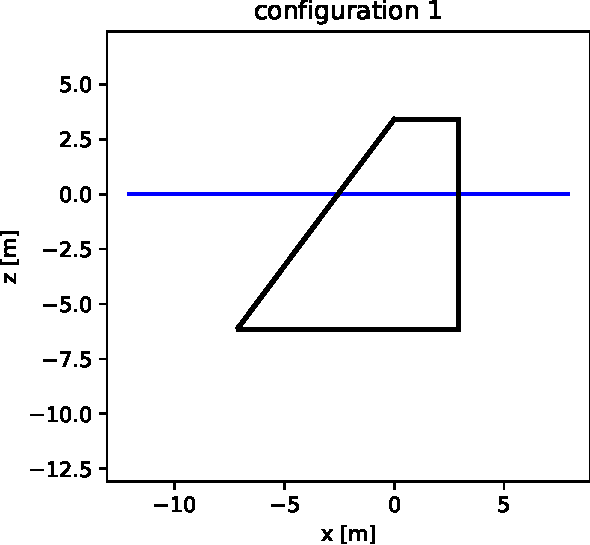
\includegraphics[width=0.475\textwidth]{figures/ComFLOW/Breakwater Geometries/Design Iteration 1 captive/top from costs/DI2/breakwater_geometry1.pdf}
    \caption{The most optimal breakwater based on costs}
    \label{fig:  most optimal breakwaters DI2 costs captive}
\end{figure}


